% !TeX root = ../report.tex
\section{Instance definition}
Before going on with reinforcement learning, we cover the underlying simulation with which the reinforcement learning agent will interact.

The simulation implements an intersection located in southern Odense, Denmark, visualized in figure 1.
Appendix A contains technical drawings of the intersection.


\subsection{Network topology}

The intersection connects an arterial road (North/South) with a collector street (East) and a gas station (west), all of which have a speed limit of 50 km/h.

\begin{figure}[!htb]
  \centering
  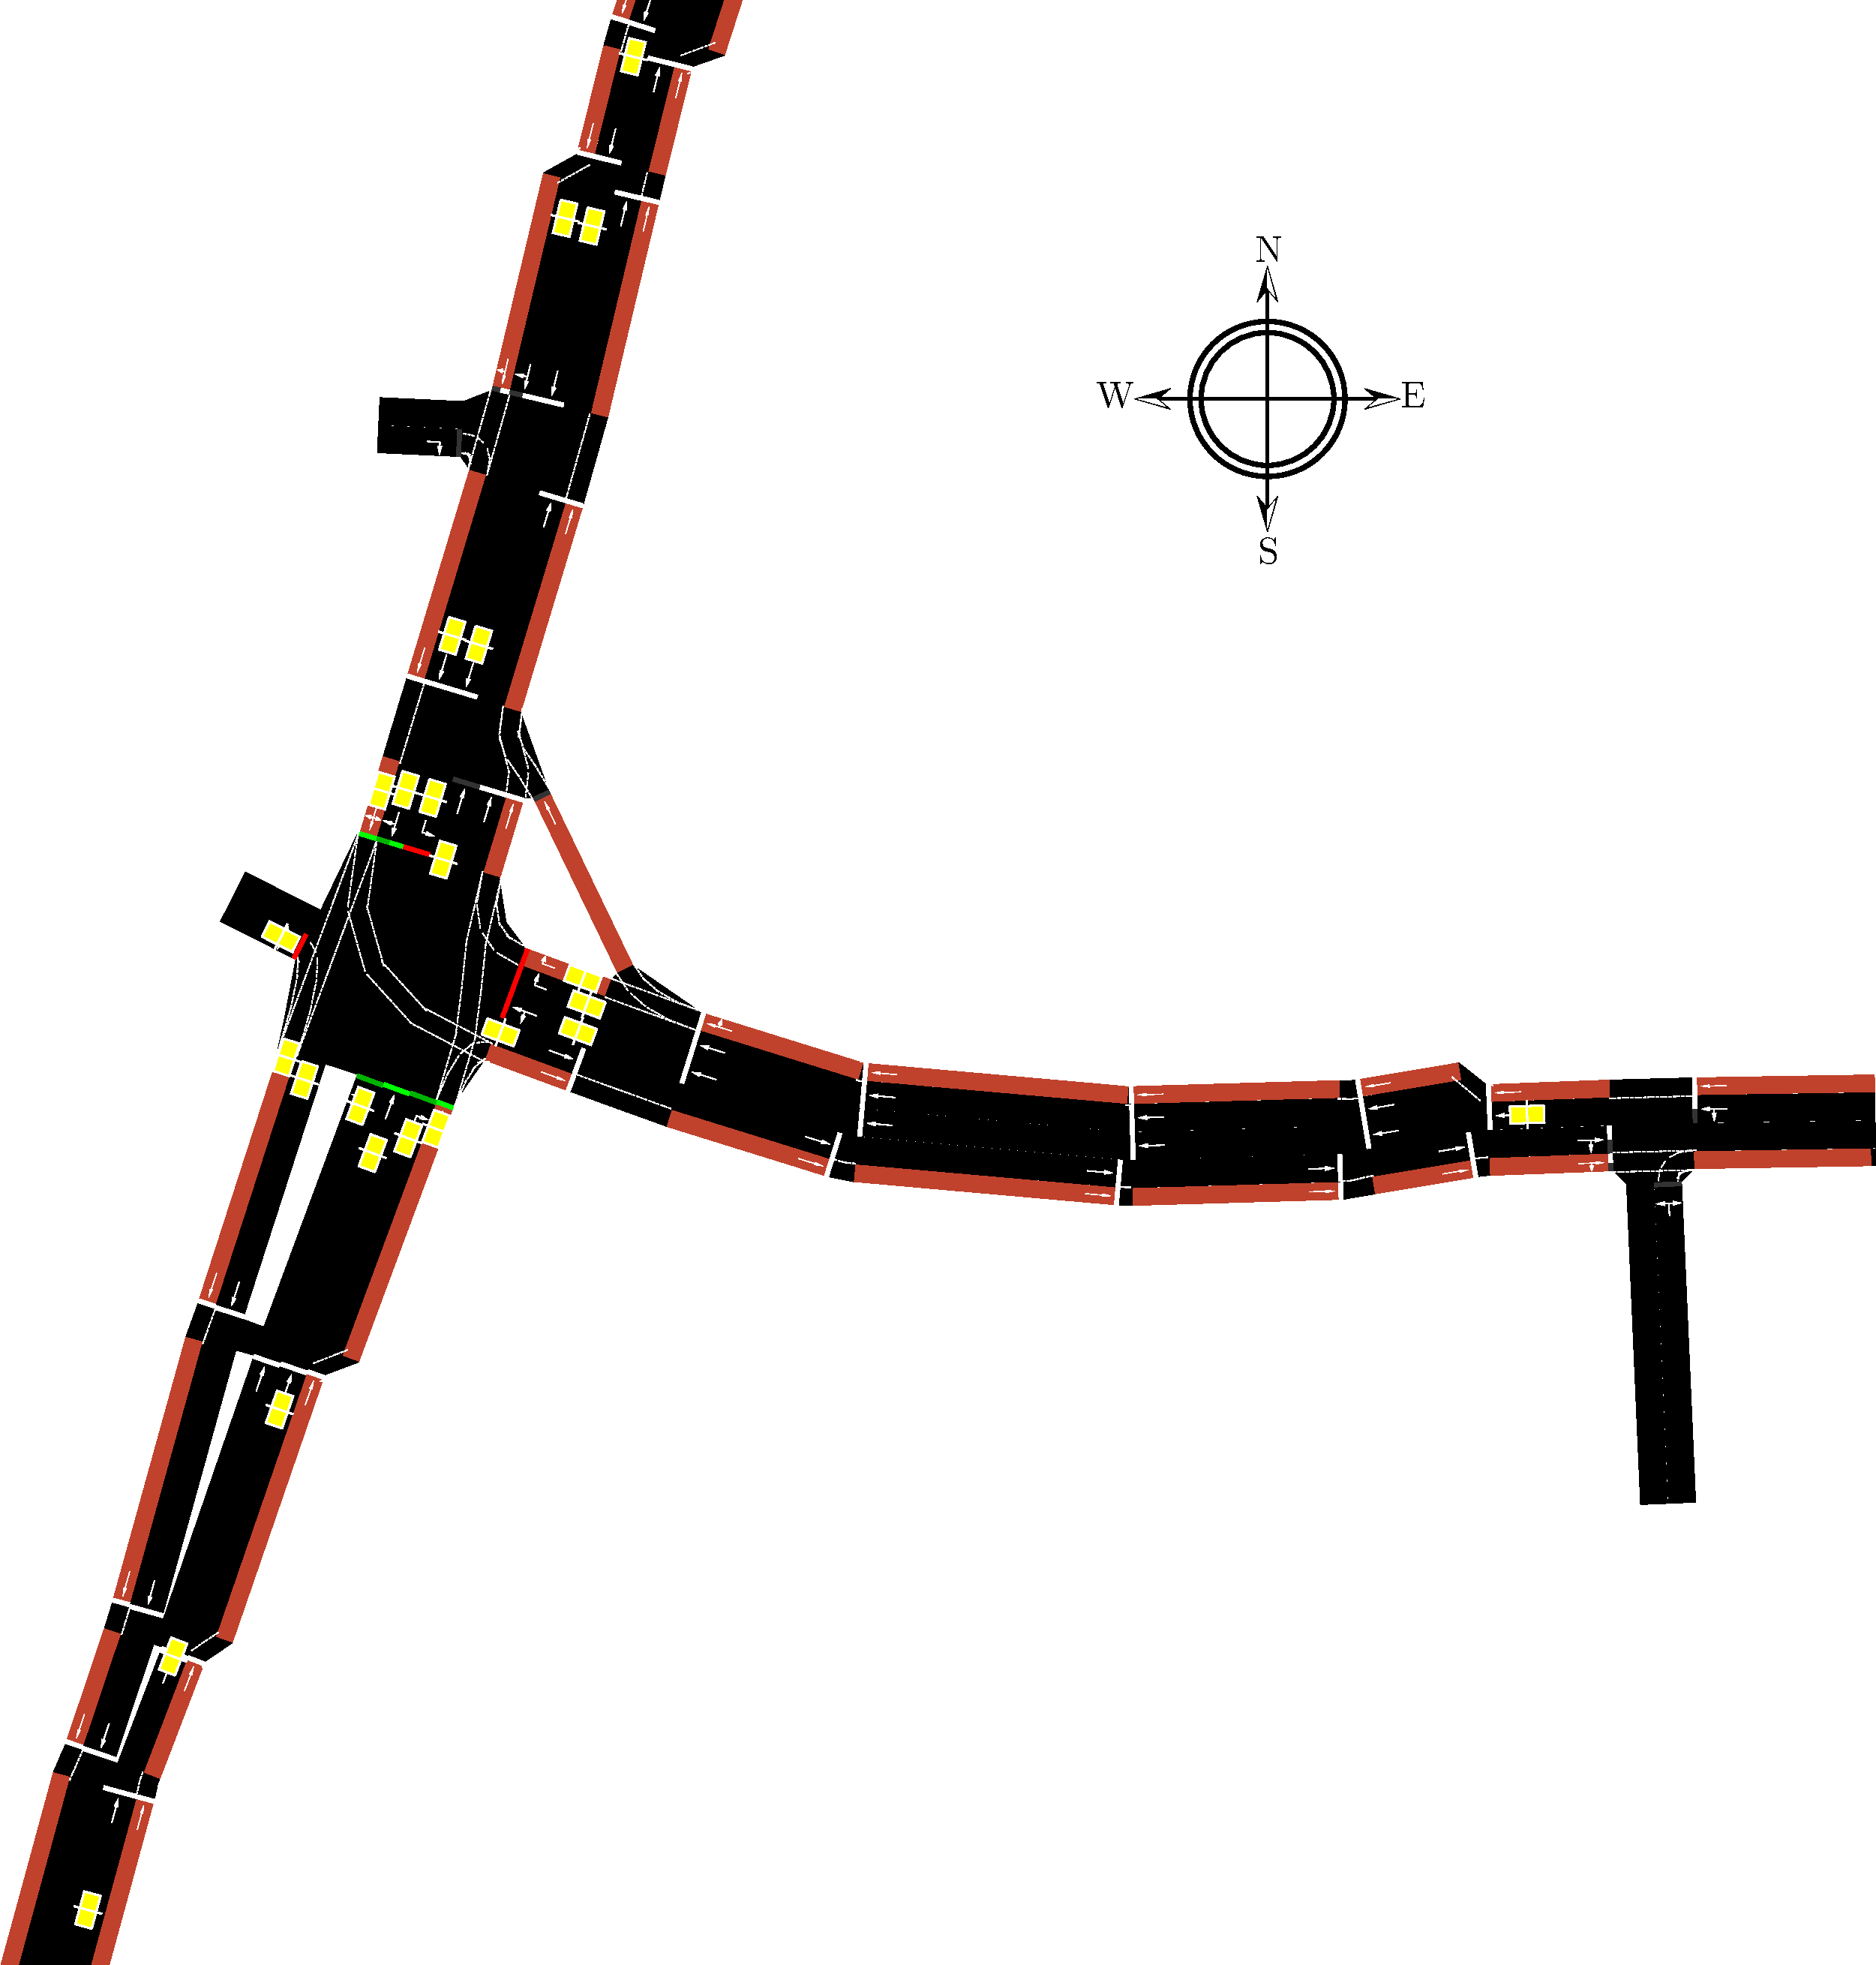
\includegraphics[scale=0.2]{../include/PDF/intersection_with_compass.pdf}
  \caption{Intersection as implemented in SUMO}
  \label{fig:sumointerimpl}
\end{figure}

\subsubsection{Induction Loops}
In the network, a number of vehicle detectors are present in the form of \textit{induction loops}, visualized in \cref{fig:sumointerimpl} as yellow boxes.

Induction loops are the only way of getting vehicle data from the traffic network, and only very few areas have more sophisticated solutions such as traffic cameras or vehicle radars. We assume that we can retrieve the following information from an induction loop, on a one-second basis:
\begin{itemize}
  \item Number of vehicles passed.
  \item Percentage of time the loop was occupied.
\end{itemize}

The induction loops in the network cover vehicles quite well, but lack when it comes to bicycles, so we exclude bicycles from the current iteration of the project.


\subsubsection{Traffic lights}
\Cref{appendix:techdraw} also contains a drawing of the traffic light layout at the intersection, from which we can derive the possible resolution of traffic control at the intersection.

The intersection implements three phases.
The first phase gives the green light to the south- and north-bound vehicles (A1 and A2), while giving \emph{conditional} green to the left and right turns of those movements (including A1v).
The second phase is only activated if vehicles occupy detectors \texttt{D23} and \texttt{D3} when the first phase goes yellow and gives the green light to southbound traffic (A1), as well as A1v and B1h. 
The third phase consists of a green light for the west- and east-bound vehicles (B1 and B2), with conditional green for left- and right turns.


\subsection{Simulator}
SUMO, short for \emph{Simulation of Urban MObility}, is a microscopic, well-established general-purpose traffic simulator. It has been around since 2001 and is an open source project. What makes it particularly interesting for this project, is the ability to control elements of the simulation externally, through a well-defined API. With this API, gathering information from the simulation for our agent is made simple, while also providing a way for our agent to control each traffic light.

SUMO uses a directed graph representation to define a traffic network, with some extra information. 
\textit{Nodes} in the graph are points connected by one or more \textit{edges}. Nodes contain connection data, which is (potentially) a many-to-many mapping of incoming lanes to outgoing lanes. The edges carry the lane information, allowing any number of adjacent lanes (within computational reason) to follow any single edge between two nodes. As such, each edge defines a set of up- or down-stream lanes, possibly consisting of multiple traffic movements.

The primary discrepancy between the actual intersection and the one implemented in this project, is the missing induction loop \texttt{D18} located in the center of the intersection. 
The induction loop is not present in the SUMO implementation as SUMO only allows placing induction loops on lanes.

\subsection{Vehicle data}

Along with technical drawings of the intersection, files describing the traffic flow exist in the form of 5 minutes aggregated readings from the 25 induction loops present in the intersection.
To use this data in a meaningful way, we define orderings of the induction loops, each of which defines a route in the network. 

We will use linear integer programming to decide which routes vehicles should follow to satisfy these induction loop readings. As the data is non-perfect we propose two different models, the first of which inserts fewer vehicles than the second. In the project we use the second model, to put higher strain on the network.

The first model assumes that the induction loops never miss any vehicles, but may overcount.
The second model assumes that the induction loops do not overcount, but may miss vehicles. 

Both models give a vehicle count for each route for a single 5-minute interval and are called once for each such period.
Solving for shorter intervals increase the network load in the simulation, we use the second model in this project.

\subsubsection{Overcounts, no misses}
Given a set of routes $R$, a set of detectors $D$, a binary route representation as defined below by $B_{ij}$, and upper bounds for \textit{total} number of vehicles passing a detector, defined below by $C_i$. 
Select the number of vehicles to follow each route, such that the number of vehicles passing each detector is maximized for all detectors, given the single constraint:
\begin{itemize}
  \item No more than $C_i$ vehicles can pass detector $D_i$, $\forall i \in \set{1, 2, \ldots, |D|}$
\end{itemize}

For convenience we define the sets $I = \set{1, 2, \ldots, |D|}$, and $J = \set{1, 2, \ldots, |R|}$.

Let $B{ij}$ be a binary constant such that:
\[
  B_{ij} = \begin{cases}
    1 & \text{if route j passes detector i}\\
    0 & \text{otherwise}
  \end{cases}\quad \forall i \in I, j \in J
\]
Let $C_i$ be an an detected number of vehicles at detector $D_i,\ \forall i \in I$
Let $x_j$ be an integer variable with a lower bound of 0, indicating the number of vehicles following route $j, \forall j \ in J$
\begin{align*}
  \begin{array}{rrcll}
    \text{Maximize} & \displaystyle\sum_{j\in J}x_j \cdot \sum_{i\in I}B_{ij}&&&\\
    \text{s.t.} & \displaystyle\sum_{j\in J}B_{ij}\cdot x_j & \leq & C_i & \qquad \forall i \in I\\
    & x_j & \in & \mathbb{N}&\qquad \forall j \in J\\
    & x_j & \geq & 0&\qquad \forall j \in J
  \end{array}
\end{align*}
The objective function maximizes the total sum of vehicles passing detectors. The outer sum sums over each route, and the second sum computes the number of detectors in the route from the outer sum.

The first constraint ensures that the sum of vehicles passing a detector does not surpass its capacity.

The second constraint ensures that the number of vehicles entering the simulation is integer.

The Third constraint ensures that the number of cars on each route must be non-negative.

\subsubsection{Misses, no overcounts}
The previous model can with a few changes be modified, such that the vehicle counts act as lower bounds rather than upper bounds.
Treating vehicle counts as lower bounds will put a more significant strain on the network, as more vehicles enter the simulation, which is desired.

\begin{align*}
  \begin{array}{rrcll}
    \text{Minimize} & \displaystyle\sum_{j\in J}x_j \cdot \sum_{i\in I}B_{ij}&&&\\
    \text{s.t.} & \displaystyle\sum_{j\in J}B_{ij}\cdot x_j & \geq & C_i & \qquad \forall i \in I\\
    & x_j & \in & \mathbb{N}&\qquad \forall j \in J\\
    & x_j & \geq & 0&\qquad \forall j \in J
  \end{array}
\end{align*}

The objective of the new model is to minimize the number of vehicles passing induction loops, while enforcing that at least the observed number of vehicles pass.

It is important to note that in this model, $B_{i\cdot}$ must contain at least $one$ $1$ to be feasible for all $i$, whereas this was not the case for the previous model.